\documentclass[a4paper, 10 pt, conference]{ieeeconf}  % Comment this line out
                                                          % if you need a4paper
%\documentclass[a4paper, 10pt, conference]{ieeeconf}      % Use this line for a4
                                                          % paper

\IEEEoverridecommandlockouts                              % This command is only
                                                          % needed if you want to
                                                          % use the \thanks command
\overrideIEEEmargins
% See the \addtolength command later in the file to balance the column lengths
% on the last page of the document



% The following packages can be found on http:\\www.ctan.org
\usepackage{graphics} % for pdf, bitmapped graphics files
\usepackage{epsfig} % for postscript graphics files
\usepackage{mathptmx} % assumes new font selection scheme installed
\usepackage{times} % assumes new font selection scheme installed
\usepackage{amsmath} % assumes amsmath package installed
\usepackage{amssymb}  % assumes amsmath package installed
\usepackage{epstopdf}
\usepackage{setspace}
\usepackage[margin=20mm]{geometry}
\usepackage{anyfontsize}
\usepackage{hyperref}
\usepackage{bm}
\DeclareMathOperator*{\argmin}{arg\,min}
\DeclareMathOperator*{\argmax}{arg\,max}
\title{\LARGE \bf Transfer}

\author{Mark McLeod}
\date{}
\usepackage{graphicx}
\begin{document}
\maketitle
\thispagestyle{empty}
\pagestyle{empty}

%%%%%%%%%%%%%%%%%%%%%%%%%%%%%%%%%%%%%%%%%%%%%%%%%%%%%%%%%%%%%%%%%%%%%%%%%%%%%%%%%%%%%%%%%%%%%%%
\section{Paper Section}
\begin{abstract}
A scheme for advance publication of electricity tariffs is proposed in which intelligent home agents optimise their behaviour to achieve minimum cost heating under the published tariff. A model of grid demand in response to tariff is developed and a Gaussian process global optimisation method used to find the tariff that minimises a cost function over the shape of the load induced. Using this procedure it is shown that the absolute flatness of the load predicted by the model can be improved by at least 12.6\% compared to that under a flat tariff.
\end{abstract}

\subsection{Introduction}

%material from \url{https://github.com/markm541374/tariffset/blob/master/problem_spec.pdf}
In order to reduce greenhouse gas emissions many governments are aiming both to reduce their energy use and to reduce the proportion of energy that is derived from unsustainable sources. This naturally means a significant increase in energy being produced by renewable sources such as solar, wind, hydroelectric, geothermal and tidal. Most of these sources provide a supply that is much less controllable, and much less reliable than traditional non-renewable supply methods. One of the key changes required to implement these changes is the development of the smart grid, in which consumers and suppliers exchange information and modify their actions in order to ensure continuous power despite uncontrollable limitations in supply. Since the ability of humans to react to price variation is limited, and certainly not sufficient to find optimal strategies for complex problems such as scheduling heating under variable tariffs and external temperatures, the use of semi-autonomous devices that are able to react to changes in the network by altering their behaviour is required \cite{rogers2012delivering} These agents will of course be primarily aiming to achieve maximum utility for the consumer, so the field of incentive engineering is required to ensure that the optimal course of action from the individual agent perspective leads to desirable behaviour in the entire system.

The current state of the electricity grid is that the electricity tariff presented to domestic consumers is either constant, or a very simple time-of-use tariff such as economy-7 and the supply adapts to meet demand. To ensure that demand is met a hierarchy of sources are used with cheaper, and more efficient, but slower responding supplies such as nuclear power are used wherever possible, and fast responding but inefficient and more expensive supplies such as gas turbines used to match variation on shorter time scales. Spinning reserves accommodate extremely fast variations and a moderate number of storage schemes such as pumped hydroelectric take up excess when required and feed it back at a later time. Supply companies buy contracts to meet any predicted demand that cannot be met with their own sources, or sell excess supply in an advance market, then pay with hindsight for the difference between this and the energy actually used by their customers.

In order to make improvement on this process it is necessary for the consumer to be made aware in some way of the availability of power and alter their behaviour by shifting consumption away from times when demand is high and towards times where there is excess capacity that would otherwise need to be stored and reintroduced with an associated losses due to ineffficiency. Previous schemes that have aimed to implement this are discussed in section \ref{reviewtariffset}. The proposed method here is to introduce a tariff that varies with time according to a parametrised generating function and is communicated to consumers ahead of time. The intelligent consumer agents then alter their behaviour to incur minimum cost under this tariff while still achieving their goals. The parameters used to generate the tariff will be selected by optimising the load profile that is induced to mave maximum flatness.
To achieve this optimisation a model of the home and the agent controlling is developed, so far only concerning heating, and an ensemble of draws from this process is used as a model of the consumer base. Evaluating the response of this model to a given tariff provides a prediction of the load and this can be used to optimise the parameters of the tariff. Results are presented showing that the optimum parametrisation of the tariff provides a significant improvement of the induced load in terms of flatness. This is an improvement over existing techniques as it achieves these improvements in load profile without requiring any cooperation, or even behaviour that is not individually optimal on the part of the consumers.

%Preamble about government energy targets, carbon, orchid, and the impending rise of the smart grid.

%Short overview of electricity generation and distribution that motivates influencing the shape of the daily load profile.

%The aim of this work is to develop a method for setting time varying tariffs in a way that allows the shape of the load profile due to domestic space heating to be controlled.
%%%%%%%%%%%%%%%%%%%%%%%%%%%%%%%%%%%%%%%%%%%%


%%%%%%%%%%%%%%%%%%%%%%%%%%%%%%%%%%%%%%%%%%%%
\subsection{The Consumer Problem}
To form a realistic model of the response to variation in tariff a realistic model of the home is required. Ramchurn et al. \cite{ramchurn2011agent} divides domestic loads into these that are and are not suitable candidates for influence via pricing. The latter are devices that are used directly by the residents such as lighting, cooking and entertainment, the former devices such as washing machines, refrigerators and heaters. This category is further split into shiftable static load (those that could start at a selection of times but once started will run a fixed profile) and thermal loads. A model for thermal loads is developed and it is these devices that are the focus of this paper. In 2012 $77.6 TWh$ of electricity was used for domestic purposes, of which $16.5 TWh$ was used for space heating \cite{ecuk_data} so thermal loads represent a significant fraction of electricity use. They also have the advantage over other devices that they are likely to be always on as a background process.

Thermostats are already getting more intelligent and are subject of recent research to produce more intelligent versions \cite{rogers2011adaptive} \cite{ramchurn2013agentswitch} with some currently available models having features such as individual room control \cite{honeywell}, highly configurable schedules \cite{nest} and occupancy detection \cite{tado}. Publication of price profiles on the internet in advance has already been proposed \cite{ramchurn2011agenthomeo}, for both real time and advance publishing. Advance publishing allows the thermostats to plan ahead but has only been proposed as predicted market price \cite{rogers2011adaptive}, not as control signal that is determined by the supplier.

The smart thermostat model presented here is based on the model proposed in \cite{rogers2011adaptive} in that it uses a quadratic utility cost for the predicted deviation from a target temperature during times when the thermostat required to be active and sums this with the cost of the power used to obtain a utility for that policy. The most notable difference between that model and the one used here is that rather than requiring the heating to be either on or off the heating control is allowed to be any value between zero and one. This assumes a pulse width modulation scheme is present in the controller, so that the control input multiplied by the heating system power gives the expectation of load rather than the true load. By doing this the duration of each control period can be increased, and so the number of degrees of freedom is reduced leading to a reduced time to complete the quadratic optimisation. It is also assumed here that the temperature cycle is periodic over 24 hours, this removes the initial value from the problem.

A simple exponential cooling model is used, the home is defined by a thermal mass, $cm$, and insulation value, $\frac{1}{k}$, and a heater power $P$ If the external temperature is $T^{e}(t)$ then the temperature is governed by the first order differential equation
\begin{equation}
\frac{dT(t)}{dt} = -\frac{k}{cm}(T(t)-T^{e}(t)) +\frac{P\delta(t)}{cm}
\end{equation}
where $\delta(t) \in (0,1)$ determines the power setting of the heater. For a sufficiently small timestep $\Delta t$  this can be approximated as an update rule
\begin{equation}
T_{n+1} =  T_{n}-\frac{\Delta t k}{cm}(T_{n}-T_{n}^{e}) + \frac{\Delta t P \delta_{n}}{cm} 
\end{equation}
If the time period under consideration is discretized into $N$ periods of $\Delta t$ then $T, T^{e},\delta$ can be represented as column vectors of size $N$ and the update rule can be expressed as a matrix equation
\begin{equation}
\left( \mathbf{I}_{N+1 \times N \times 1}-(1-\frac{\Delta t k}{cm})\mathbf{U}\right) \underline{T} = \frac{\Delta t k}{cm}\mathbf{U}\underline{T}^{e}+\frac{\Delta t P}{cm}\underline{\delta}
\end{equation}
which is an affine relation between temperature and input that can be expressed as

\begin{equation}
\underline{T}=\underline{\Psi}+\boldsymbol{\Phi} \underline{\delta}
\end{equation}
where
\begin{equation}
\boldsymbol{\Phi}= \frac{\Delta t P}{cm} \left( \mathbf{I}_{N+1 \times N \times 1}-(1-\frac{\Delta t k}{cm})\mathbf{U}\right)^{-1}
\end{equation}
\begin{equation}
\underline{\Psi}= \left( \mathbf{I}_{N+1 \times N \times 1}-(1-\frac{\Delta t k}{cm})\mathbf{U}\right)^{-1} \left( \frac{\Delta t k}{cm}\mathbf{U}\underline{T}^{e}\right)
\end{equation}
and
\begin{equation}
\mathbf{U} = \left[
\begin{array}{c|c}
\underline{0}_{1\times N} & 1 \\ \hline
\mathbf{I}_{N} & \underline{0}_{N \times 1}
\end{array}\right]
\end{equation}

The quantity that the home controller needs to minimise is the sum of the cost of deviation from the target temperature profile $\underline{T}^s$ and the cost of heating integrated over the 24 hour period. The temperature deviation is only relevant when the home is occupied. This is encoded in the matrix $\mathbf{Q}=q \times diag(\underline{o})$ where $\underline{o}$ is a vector of size $N$ with ones in positions where the home is occupied and zeros otherwise and $q$ is a scalar that relates the utility of temperature deviation to monetary cost. The cost of heating is given by $P\underline{\Lambda}^{T} \underline{\delta}$ where $\underline{\Lambda}=[ \lambda ]$ is the vector of size $N$ giving the unit cost of electricity over time. This gives an objective function

\begin{equation}
f = (\underline{T}-\underline{T}^s)^{T}\mathbf{Q}(\underline{T}-\underline{T}^s)+P\underline{\Lambda}^{T} \underline{\delta}
\end{equation}

So that the dimensionality of the problem can be reduced to a reasonable value for the optimisation stage while still maintaining a good resolution in the thermal simulation the raw control input, $\underline{\delta}$ is defined to be
\begin{equation}
\underline{\delta}=\mathbf{D}\underline{u}
\end{equation}
where $\underline{u}$ is the $M$ dimensional column vector that will be optimised over and $D$ is the $M\times N$ matrix
\begin{equation}
\label{quadthermodimension}
\mathbf{D}=\mathbf{I}_{M} \otimes \underline{1}_{J \times 1},\qquad \emph{s.t.} \quad N=MJ
\end{equation}
This allows each element of the new control input, $\underline{u}$ to be mapped to $J$ elements of $\underline{\delta}$.

Making these substitutions leads to the new objective function
\begin{equation}
\label{furuus}
f'=\underline{u}^{T}\mathbf{R}\underline{u}+\underline{S}^{T}\underline{u}
\end{equation}
where
\begin{equation}
\mathbf{R}=\mathbf{D}^{T}\boldsymbol{\Phi}^{T}\mathbf{Q}\boldsymbol{\Phi}\mathbf{D}
\end{equation}
and
\begin{equation}
\underline{S}^{T}=2(\underline{\Psi}-\underline{T}^s)^{T}\mathbf{Q}\boldsymbol{\Phi}\mathbf{D}+P\underline{\Lambda}^{T} \mathbf{D}
\end{equation}
Which differs from the original objective by a constant.

The only constraints strictly required are those that constrain the heater input to be set between zero and one. 
\begin{equation}
0 \leq \delta_{n} \leq 1 \qquad \forall n
\end{equation}
These are expressed in standard form as
\begin{equation}
\left[
\begin{array}{c}
\mathbf{I}_{M} \\ \hline
- \mathbf{I}_{M} 
\end{array}\right]\underline{u} \leq \left[\begin{array}{c}
\underline{1}_{M \times 1} \\ \hline
\underline{0}_{M \times 1}
\end{array}\right]
\end{equation}
In the following results two further constraints are also placed. An absolute maximum and minimum temperature over all time are introduced, assuming that even when not present in the home some constraints will be desired, and an upper limit to the deviation from the target temperature is placed, assuming that the user will want the temperature reasonably close to the target despite any savings that might be available.

An example of the heating profile produced is shown in figure \ref{quadtemp}. Under a flat tariff the temperature profile would fall at the end of the active periods and remain at the minimum unlit the latest time that the heating must turn on to return to the target for the start of the next period. The tariff shown is a cubic spline fitted to nine support points and clearly causes the initial load required to heat the house in the morning to be shifted earlier to avoid the rising slope of the tariff at that time.

\begin{figure*}[htb]

\centering
\includegraphics[width=\textwidth,trim =4cm 8cm 4cm 2cm,clip=True]{f4.eps}
\caption{Home heating under a variable tariff over a 24 hour period. The upper plot shows temperature demand (green), actual temperature (blue) and external temperature (red). The middle plot shows the power consumption, the lower plot shows tariff. The shape of the tariff has caused the optimum  heating strategy to be to heat to above the target temperature ahead of time in the morning.}
\label{quadtemp}
\end{figure*}

The above specifies the procedure an individual smart thermostat will undertake to form an optimum heating plan given its operating constraints. To perform this optimisation over a 24 hour period using 15 minute intervals periods and 1 minute cooling simulation with he code used in the results below requires approximately three seconds as a single threaded process on an Intel i7 processor. This leads to the set of 60 agents used for tariff optimisation taking approximately 40 seconds to find the response to a given tariff. The results show that 60 agents still have significant differences in response between draws meaning greater numbers would be desirable. Therefore this is clearly a sufficiently expensive to evaluate objective to justify the use of the techniques described below. 
%%%%%%%%%%%%%%%%%%%%%%%%%%%%%%%%%%%%%%%%%%%

\subsection{The Supplier Problem}
In this work we consider an electricity supplier with a set of customers $c \in C$. Each of these customers has a load $l_{c}(t)$  so that the load to be met by the supplier is
\begin{equation}
L(t) = \sum_{c \in C} l_{c}(t)
\end{equation}
There exists some utility functional for production $U_{p}(L(t))$ which specifies how much it costs the producer to supply this power. $U$ will be based on the sources of power and their operational costs available to the supplier, and the market prices at which it must sell excess and buy shortfall.
Each consumer is charged at a rate which is defined to be some function of time $\lambda (t)$. The balance of payments for the supplier is therefore
\begin{equation}
\Delta = \int_{T}L(t) \lambda(t) \mathrm{d}t - U_{p}(L(t))
\end{equation}
and the supplier naturally wishes to choose $\lambda$ to maximise profit (subject to constraints such as not being so high that consumers will choose to use other supplies). To simplify the mathematics for this work it is assumed that the income collected due to the tariff will balance the component of $U$ which is due to the average power consumption, so are only concerned with the shape of $L$ rather than its absolute value. The following results use the integral of absolute difference from the mean power, but other options are of course available and are discussed in section REF.
Further, the load is divided by end use into load that is and is not controllable via $\Lambda$ and only that component which is controllable is considered.

To model the response of the full set of customers multiple agents are created using a generative process to determine individual parameters and the sum of their load is used. That is is a single thermal agent from the set of agents in the ensemble $a \in A$ is characterised by a vector $\theta_{a}$ and the optimisation process that produces a load profile $\underline{l}$ given a tariff profile $\underline{\Lambda}$ is denoted
\begin{equation}
\underline{l}=h(\underline{\Lambda} \mid \theta)
\end{equation}
then the load $\underline{L}$ produced by the entire ensemble of agents is
\begin{equation}
\underline{L}(\underline{\Lambda}) = \sum_{a \in A} h(\underline{\Lambda} \mid \theta_{a})
\end{equation}
To provide an suitable target for optimisation the load profile vector must be mapped to a scalar that conveys the utility to the supplier of that load. For the following results the objective used is the normalised integral of the deviation from the mean load.
\begin{equation}
U(\underline{L})=\sum_{t=0}^{N} \frac{\left| \underline{L}[t]-\langle L \rangle \right|}{\langle L \rangle}
\end{equation}
Various other possibilities are discussed in section \ref{reviewtariffset}.

There is of course the possibility that a tariff might exist which exactly flattens the load and which can be found in a deterministic manner. For a single agent this would mean a constant power draw and if a value exists that satisfies the agent constraints then the tariff that induces this behaviour can be found by setting the derivative of equation \ref{furuus} with respect to $\underline{u}$ to and rearranging to obtain
\begin{equation}
\label{flattar}
\underline{\Lambda} = -\frac{1}{P}\left( 2\mathbf{R}\underline{u} + 2(\underline{\Psi}-\underline{T}^s)^{T}\mathbf{Q}\boldsymbol{\Phi}\mathbf{D}\right)^{T}\mathbf{D}^T(\mathbf{DD}^{T})^{-1}
\end{equation}
However, this problem grows with the number of agents so will become intractable with larger numbers of agents, and since $\underline{\Lambda}$ must satisfy equation \ref{flattar} for some constraint satisfying $\underline{u}$ for every agent present, and maintain the sum of all agent loads exactly flat there is no reason to believe that a solution will exist for non-trivial numbers of agents. Optimising to move the load as close as possible to the desired shape is therefore the best that is likely to be achieved. Further the tariffs that would be found if unconstrained are highly likely to contain extremely high and low values at critical times which would not be acceptable in reality. The tariff is therefore constrained to lie within reasonable bounds in the following simulations.
%%%%%%%%%%%%%%%%%%%%%%%%%%%%%%%%%%%%%%%%%%%%%%%%%%%%%
\subsection{thermal agent generative process}
In order for the model to provide useful information it must have similar characteristics to the true demand system. Creating a model with structure and parameters sufficiently well chosen to provide responses that are close to reality is discussed in section REF. For this work more simpler distributions, and nominal values have been used to provide a model that can be used for optimisation and is hopefully not too dissimilar to reality. The full set of parameters used are listed in table \ref{modelpara}

To determine the times that the home must be maintained at the desired temperature the work of \cite{richardson2008high} is used. They propose a Markov chain generative model based on survey data. The model provides transition matrices for the number of active occupants in a building every ten minutes throughout the day, with separate chains for buildings with between one and six occupants. For this it is required to specify the number of occupants living in the building. For this a discrete distribution is used, based on data collected in the CABE dwelling size survey \cite{CABE} which lists the number of occupant for 200 English homes.

\begin{table}[h]
\caption{Parameters of Home Model and their Distribution}
\label{modelpara}
\begin{center}
\begin{tabular}{|c||c|}
\hline
Parameter & Model\\
\hline \hline
Occupancy Number & Multinomial \\
\hline
Occupancy over time & Markov-Chain \\
\hline
Floor area (A) & Offset Gamma \\
\hline
Flat or House & Binomial  \\
\hline
Insulation Value (House) & $3.6\sqrt{A}+0.14A$\\
\hline
Insulation Value (Flat) & $3.3\sqrt{A}$\\
\hline
Electric Boiler Power & Uniform\\
\hline
Thermal Capacity & Log-Normal  \\
\hline
Maximum Temperature & Normal \\
\hline
Minimum Temperature & Gamma \\
\hline
q & Log-Normal \\
\hline
Maximum Deviation from Target & constant \\
\hline
\end{tabular}
\end{center}
\end{table}

For the thermal parameters of the home the floor area is drawn from an offset gamma distribution chosen to match the floor area results found by the CABE survey as shown in figure \ref{GIA} Nominal values are used to convert floor area to surface area and from these values to derive insulation and thermal mass values which are drawn from log-normal distributions based on the nominal values given in The Government’s Standard Assessment Procedure for Energy Rating of Dwellings \cite{SAP}. Future improvements to this procedure are discussed in section \ref{utilityofloading}

\begin{figure}[htb]
\centering
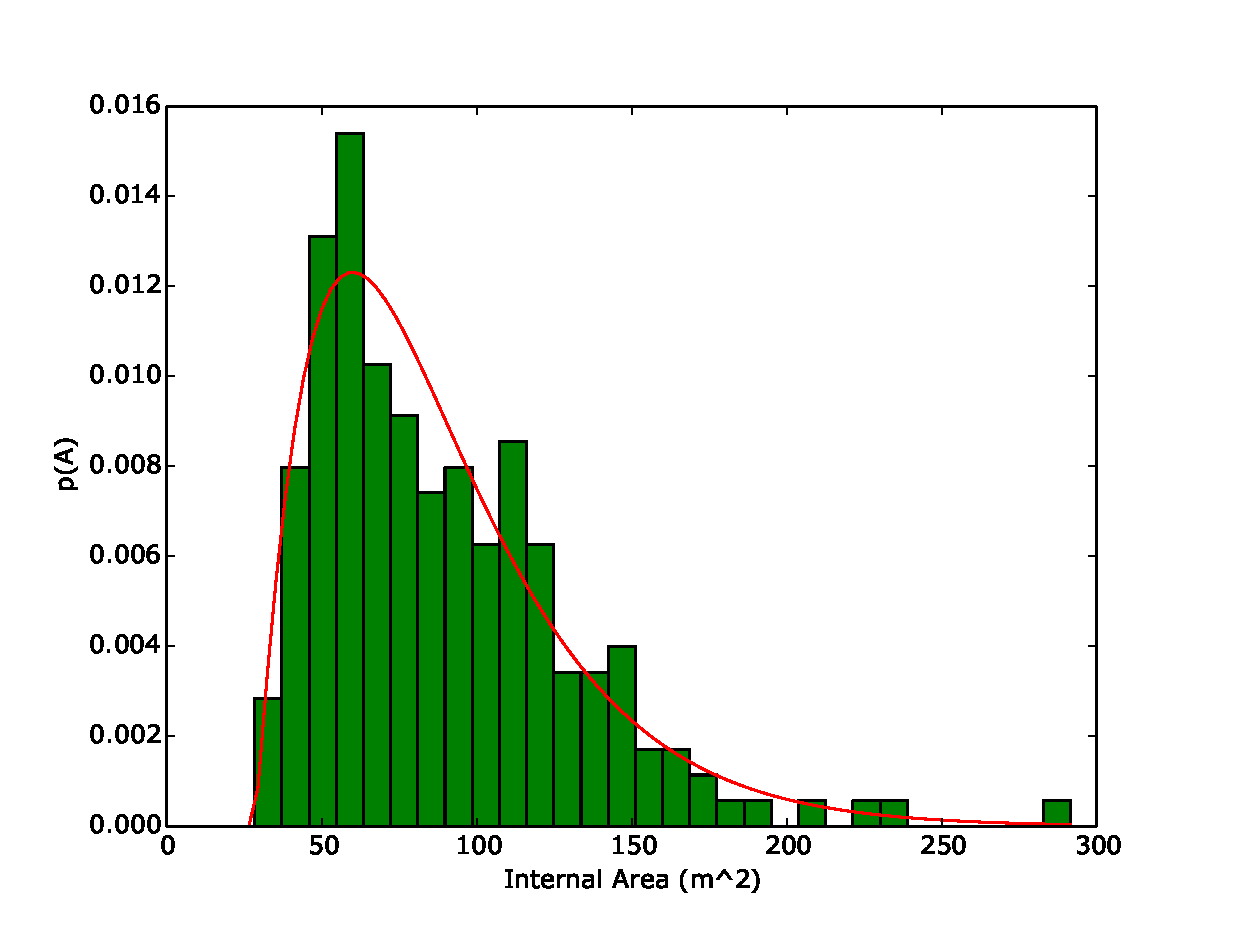
\includegraphics[width=\columnwidth,trim =0cm 0cm 0cm 0cm,clip=True]{f3.eps}
\caption{The internal floor area of a home. The histogram shows data obtained from the CABE study. This has been fitted to an offset Gamma distribution with $shape=2.10$, $scale=28.70$, and $ offset=28.39$ shown in red. The mean and variance of the histogram and the fitted Gamma distribution are equal, the offset it that which minimised the squared error between the Gamma distribution and the histogram at the bin centres.}
\label{GIA}
\end{figure}

%%%%%%%%%%%%%%%%%%%%%%%%%%%%%%%%%%%%%%%%%%%
\subsection{Optimization}
Combining the supplier and consumer definitions the objective function we with to evaluate is
\begin{equation}
g = U(\underline{L}(\Lambda))
\end{equation}
Rather than search over the full N dimensional space of $\Lambda$ we specify the tariff to be smoothly varying and defined by some parametrised function $\lambda(t \mid \theta)$. The search then takes place over the much smaller space defined by $\theta$. For the following results we interpret $\theta$ as equally spaced support points of a cubic spline over the period, with an additional constraint that the tariff is bounded above and below by some maximum and minimum value. Various other possibilities are of course available.

Since the function, $g$, we with to optimise involves the solution to a constrained multidimensional quadratic for each agent in the ensemble it requires significant computing time to evaluate. It is therefore worthwhile to invest some additional computing time in selecting the next point to evaluate, rather than following grid-search or multi-start line-search algorithms. The method used is Gaussian Process Global Optimisation (GPGO)\cite{garnettgaussian}, in which given a mean and kernel function a value for the expectation and variance can be obtained for any point in closed form given the points that have been evaluated and used to obtain a utility for a proposed evaluation at that point.
Specifically, when evaluating a function $y=f(\underline{x})$  it is assumed that the value of y has a prior given by $\mu (\underline{x})$ and is jointly Gaussian at all points with the covariance between two locations $x$ and $x'$ defined by a valid kernel function $k(\underline{x},\underline{x}')$. Given a set of points $\mathbf{x}_{0}$ that have been evaluated as $\underline{y}_{0}$ then the posterior distribution over the value of the function, $p(y_{s})$ at a point of interest $\underline{x}_s$ is normally distributed
\begin{equation}
 y_{s}\mid \underline{x}_{0},y_{0}\sim\mathcal{N}\left( \langle y_{s}\rangle ,\mathrm{var}(y_{s})\right)
\end{equation}
where
\begin{equation}
\langle y_{s}\rangle 	=\underline{K}_{sx}\mathbf{K}_{xx}^{-1}y_{0}
\end{equation}
\begin{equation}
\mathrm{var}\left(y_{s}\right)	=K_{ss}-\underline{K}_{sx} \mathbf{K}_{xx}^{-1} \underline{K}_{sx}^{T}
\end{equation}
\begin{equation}
K_{ss}	= k(\underline{x}_s,\underline{x}_s)
\end{equation}
\begin{equation}
\underline{K}_{sx}	=[k\left(\mathbf{x}_{0}[i],\underline{x}_s\right)]
\end{equation}
and
\begin{equation}
\mathbf{K}_{xx}	=[k\left(\mathbf{x}_{0}[i],\mathbf{x}_{0}[j]\right)]
\end{equation}

In implementation the Cholesky decomposition of $K_{xx}$ is used rather than the inverse in order to reduce computing time and avoid numerical problems.
The expectation and variance of the posterior of the function can be combined to provide some metric for the utility of an evaluation at that point. The utility used here is the expected improvement (E.I.) of evaluation at the proposed point compared to the minimum so far observed, which is defined as
\begin{equation}
EI(\underline{x}_{s} \mid \mathbf{x}_0, \underline{y}_0, k)= \int_{-\infty  }^{y_{opt}} (y_{opt}-y_{s})p(y_{s}) \mathrm{d}y_{s}
\end{equation}
where
\begin{equation}
y_{opt} = \min(\underline{y}_{0})
\end{equation}
The choice of mean and kernel and utility functions and the hyperparameters of the kernel function and their prior of course have a major influence on the effectiveness of the optimisation. In the results presented below a zero mean function and E.I. utility function have been used. For the kernel a squared exponential function has been used with independent log-normal priors over the hyperparameter values. The hyperparameters are updated under to the maximum posterior values given the observed points between evaluations. Searching for the maximum E.I. location, and for the hyperparameter values is done using the DIRECT search algorithm \cite{jones1993lipschitzian}. Alternatives to these choices are discussed in section \ref{reviewoptimisation}.
%%%%%%%%%%%%%%%%%%%%%%%%%%%%%%%%%%%%%%%
\subsection{Results}
The tariff is chosen to be a generated by a cubic spline passing through equally spaced support points. The support points are constrained to lie between five and 40 pence per kWh. Since when adjacent support points have a large difference this leads to a curve that can go considerable outside the range the tariff is also clipped so that it remains between five and 40 pence per kWh. The tariff is tested on a set of 60 models of a home created from a generative model with parameters drawn independently according to the distributions shown in table \ref{modelpara}. These agents optimise their load profile while still fulfilling their constraints using a 15 minute resolution for the control input, and a one minute resolution for cooling simulation, that is in equation \ref{quadthermodimension} $N=1440$ and $M=96$. The utility of the induced load is the negative of the sum of the difference from the mean load over the day, normalised against the mean load. Intuitively this would mean that while a continuous unit load would have a utility of zero a load of two units for half the time and zero for the rest would have a utility of $-1$.



A squared exponential kernel is used in the Gaussian process. Inputs are expressed in pounds per kWh so the  prior over input scales are chosen to be lognormal distributions centred on $10^-1$ with standard deviations of one decade. The prior over the output scale is also lognormal, with a mean of $10^0$ and a scale parameter of $1$. The optimisation is permitted to run for $250$ evaluations of the objective. The first twelve points are selected with at random to initialise the GP, with independent uniform distribution over the support points. The covariance is then updated to the MAP estimate after the initialisation. Since the evaluation of the kernel likelihood required a cholesky decomposition the time required grows rapidly with the number of points evaluated. The hyperparameters are therefore only optimised once for every ten evaluations of the objective up to the first 80 evaluations, and every 15 thereafter. In both searching for hyperparameters and for expected improvement the DIRECT algorithm is used.

\begin{figure}[htb]
\centering
\includegraphics[width=\columnwidth,trim =0cm 0cm 0cm 0cm,clip=True]{f2.eps}
\caption{The performance in terms of deviation from the mean load of the best cubic spline tariffs obtained with varying degrees of freedom on the training set of 60 agents (blue) and on a test set also of 60 agents (red). The tariff is constrained between 5 and 40 pence per kWh. Four is the minimum number of support points required to define a cubic. The horizontal lines shows the response to a flat tariff, the value taken by the flat tariff affects the response by only 1\% over the full range of 5 to 40 pence per kWh.}
\label{DOFplot}
\end{figure}

Figure \ref{DOFplot} shows the performance improvement using the best tariff found at various degrees of freedom for both test and training data. A tariff with four degrees of freedom provides a $6.7\%$ improvement of the objective function compared to a flat tariff, seven degrees of freedom allow the greatest observed improvement in the training set of $12.6\%$ improvement. It is clear that the use of the variable tariff has caused the induced load to be flattened, and this flattening is increased with more degrees of freedom in the tariff. It is worth noting that it is quite likely that there is further improvement available with further searching about 7 degrees of freedom where the curve begins to flatten, as for these searches the expected improvement available at the final point evaluated was orders of magnitude greater than the final evaluation of the searches in lower degrees of freedom. The 4 DOF search actually terminated before 250 evaluations since the expected improvements at all points tested by the DIRECT search was less than the numerical precision and evaluated as zero. This trend is also present on a test set of equal size, which demonstrates that the optimisation is not over fitting the tariff to the individual agents in the test data. 

\begin{figure*}[htb]

\centering
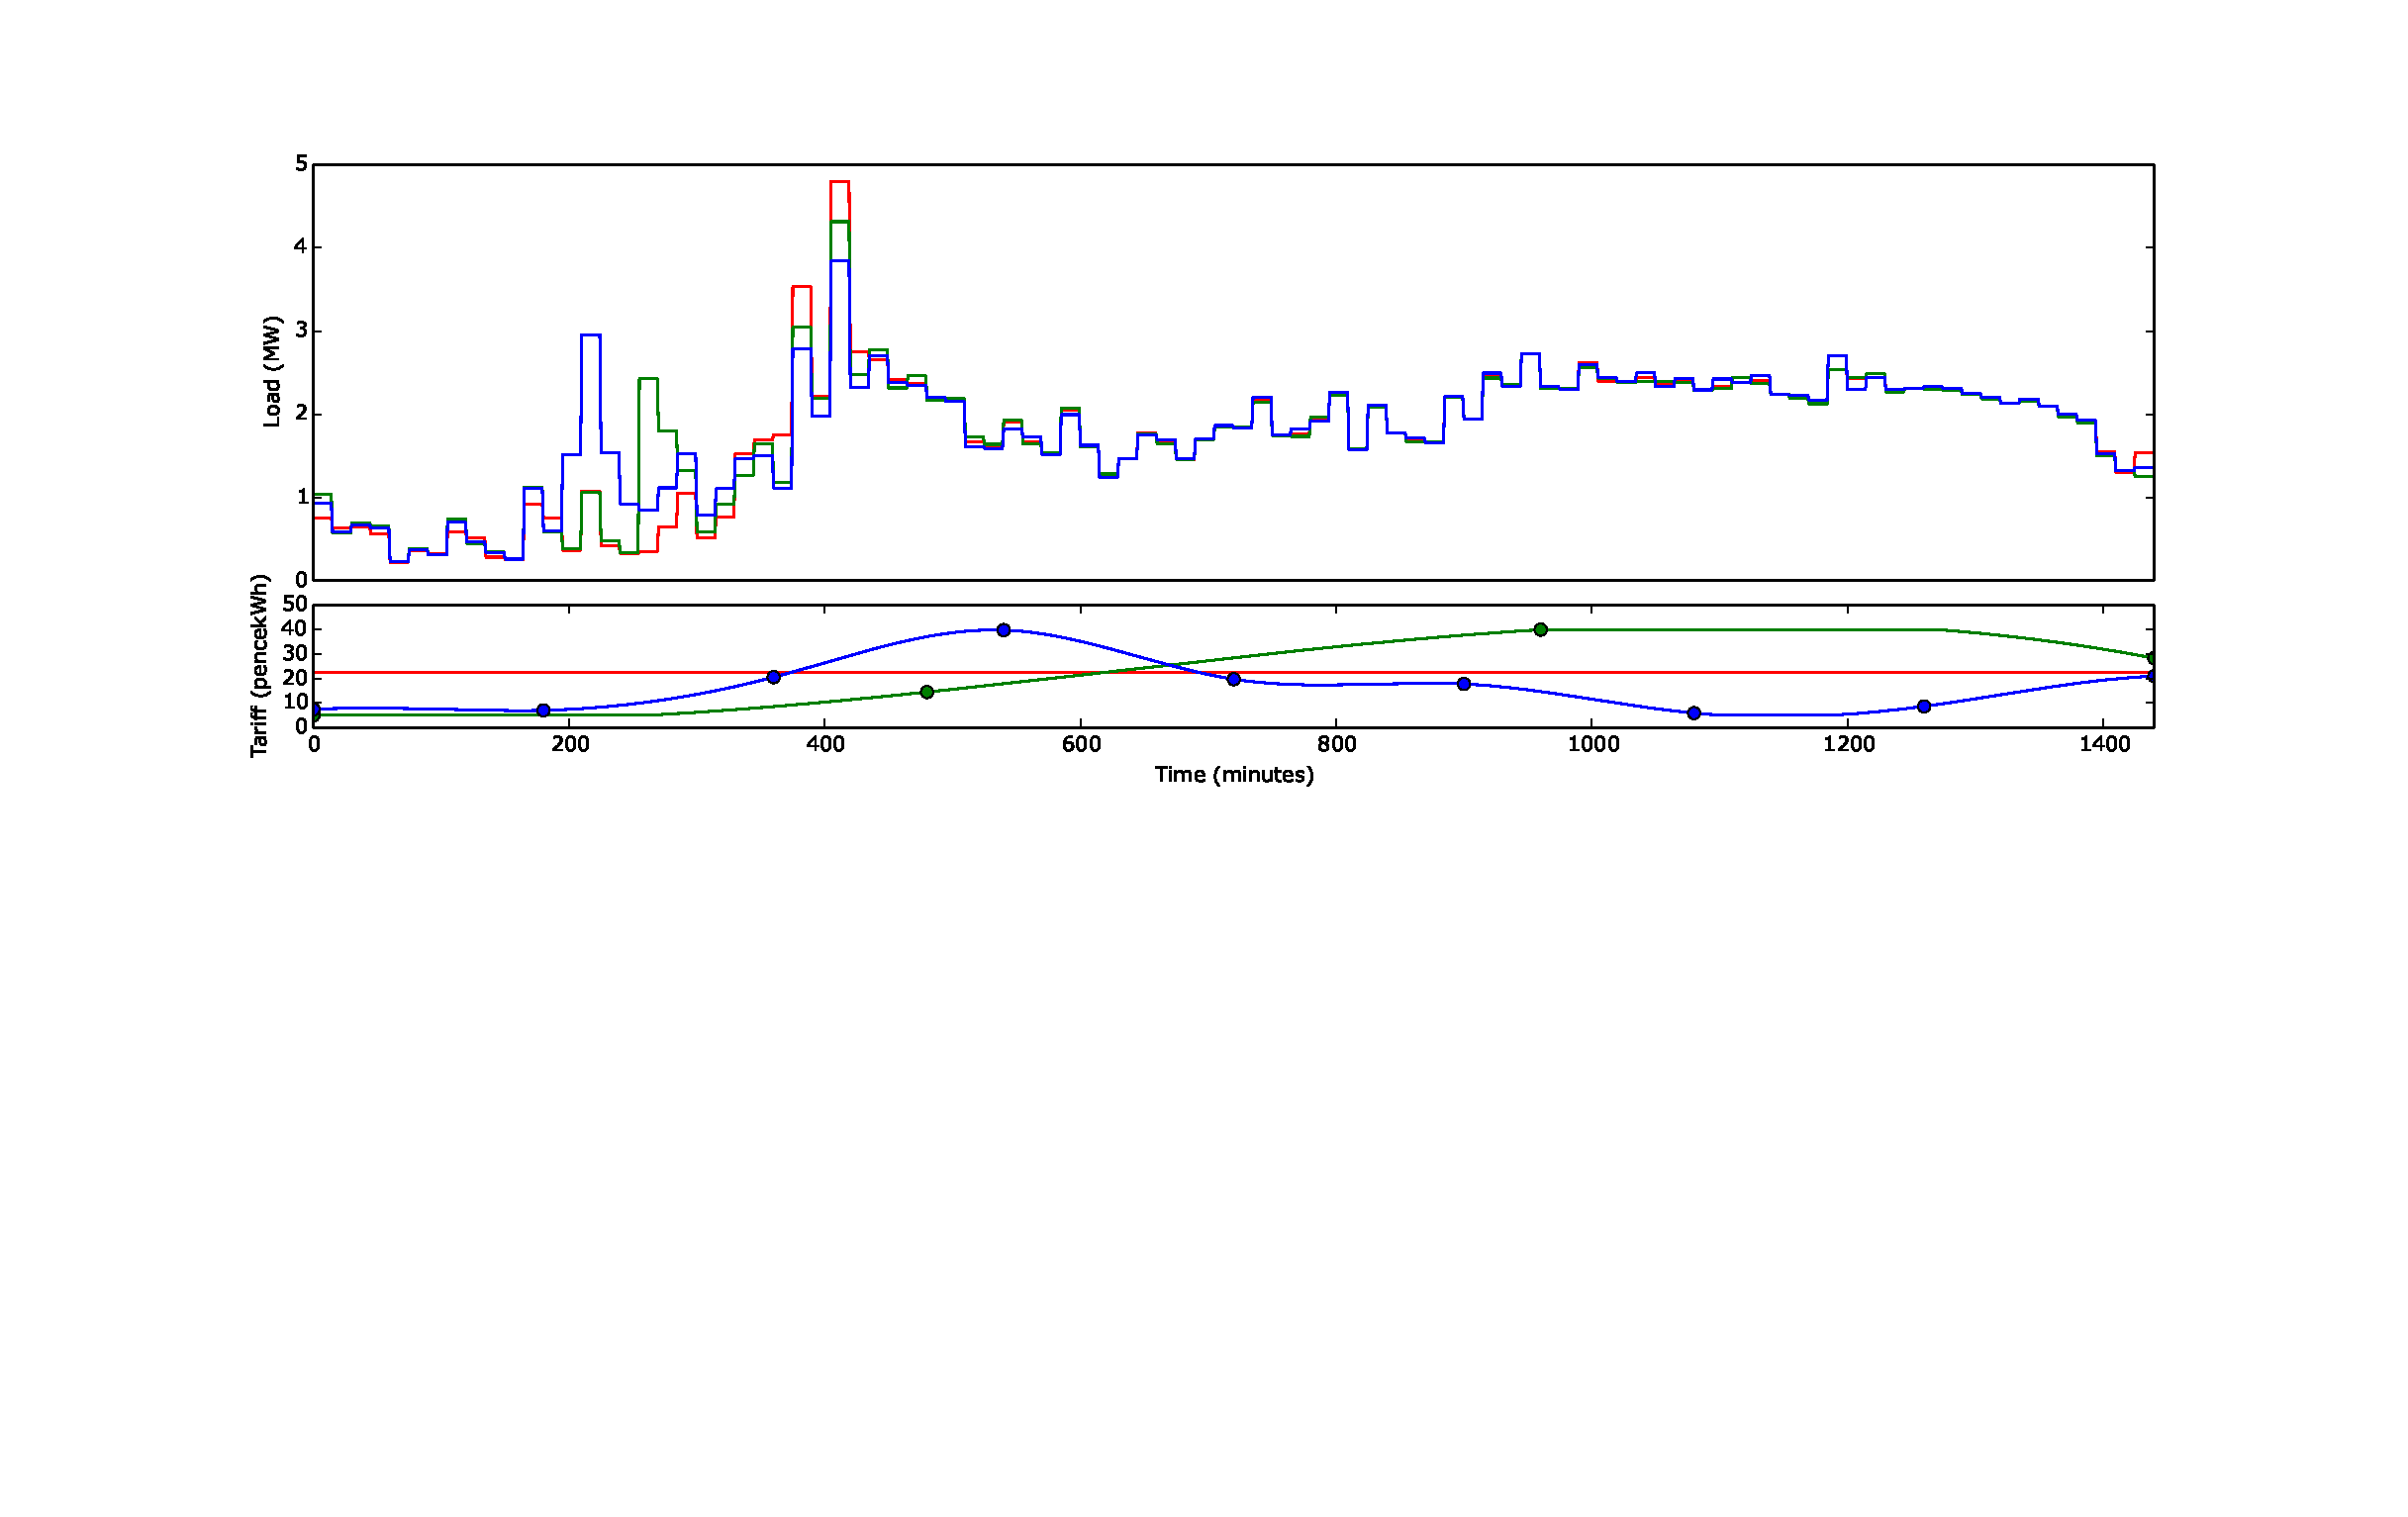
\includegraphics[width=\textwidth,trim =4cm 12cm 4cm 2cm,clip=True]{f1.eps}
\caption{Load response of an ensemble of 60 agents to variable tariffs. The upper axis shows the load in MW while the lower axis shows the tariff in pence per kWh with support points shown as filled circles. Red is a flat tariff for reference, green is the best tariff found using four support points, blue is the best tariff found using nine support points.}
\label{loadcurve2}
\end{figure*}

Figure \ref{loadcurve2} shows the load curves over the day. It can be seen that the load with a flat tariff begins at about $1MW$ until roughly 7am where there is a significant spike of roughly $4.5MW$ following which it returns to a reasonable flat $2.5MW$ for the rest of the day. The optimised tariffs make significant reductions in the peak of the spike in the morning  by shifting this load earlier.


Normally it would be appropriate to compare the price paid by the consumers under the optimised tariff to the price under the flat tariff to determine whether there is an incentive to switch. However, the response of the objective function is primarily to the shape of the tariff rather than to the value. This means that the utility of the response under a flat tariff at the maximum value of $40 pence /kWh$, which would of course lead to all consumers making savings, is only $1\%$ different from the flat response at at the minimum tariff of $5 pence /kWh$, in which case all consumers would pay more. It is therefore clearly possible to ensure that customers would prefer to select a variable tariff by appropriate selection of the value of the flat-tariff alternative. To find the truly optimal tariff it is necessary to attach a realistic to the coefficient to the distributor of non-flatness and sum this with the tariff collected from the consumers to find the real cost of a given load. This is discussed in section \ref{reviewtariffset}.

\subsection{Conclusion}
A probabilistic model for the thermal behaviour and requirements of a domestic home, and an intelligent agent that can calculate optimal behaviour for the home given a continuously varying tariff have been defined. Using a training set drawn from this model it has been demonstrated that the shape of the electrical load responds to variations in the shape of the tariff. Using a parametrised tariff a global optimisation method suited for expensive evaluations has been used to find the tariff parameters that maximise the flatness of the induced load for varying degrees of freedom, and it was found that the improvements obtained increased with increased degrees of freedom in both training and evaluation data. At best using nine degrees of freedom in the tariff the load profile was improved by $12.6\%$ in terms of absolute difference from the mean compared to the loading under a flat tariff. At this number of degrees of freedom further improvements still appeared to be available at the end of the time allocated for optimisation. It is therefore concluded that searching for variable tariffs is a feasible method for influencing the shape of the load, and that it is worthwhile to develop both the model and the search technique with the aim of achieving a model that is sufficiently similar to real consumer behaviour, and searching that is sufficiently efficient that tariffs can be proposed for real application in reasonable time. 


\bibliography{trans.bib}

\bibliographystyle{ieeetr}


%%%%%%%%%%%%%%%%%%%%%%%%%%%%%%%%%%%%%%%%%%%%%%%%%%%%%%%%%%%%%%%%%%%%%%%%%%%%%%%%%%%%%%%%%%%%%%%%%%%%%%%%
\onecolumn
\large
\section{Review/Proposal}
\doublespacing
\subsection{Intro}
In this section the two principal areas of the above work, the application of setting electricity tariffs and the global optimisation of expensive objectives are reviewed and proposals made for further research.
In the tariffsetting application the existing methods for demand management are reviewed, and compared to the method proposed above. The additional information and complexity required to produce a model that can be compared to the real grid is highlighted.
In the area of optimisation existing methods are reviewed, and it is noted that they do not strictly follow the correct decision process for optimal behaviour, and that no quantitative information about the relative performance of different algorithms is available. An possible approach to optimisation that satisfies these requirements is proposed as the subject of future research.


\subsection{Reviewtariffsetting}
\label{reviewtariffset}
A selection of potential methods for managing the demand profile from domestic electricity consumption have been proposed. Ramchurn et al. \cite{ramchurn2011agenthomeo} propose a method of homeostatic control, in which the consumer is sent a signal containing both a carbon intensity prediction, and a target for consumption relative to the same time the previous day. The agent then adapts its schedule for charging and discharging local storage to achieve a minimum cost load profile. Under this scheme the carbon emission of the system is reduced by $25\%$ and the consumer costs by up to $14.5\%$. This is not completely desirable since it relies on the consumer being willing to subscribe to a scheme which aims to reduce cost weighted against with carbon emission rather than the absolutely cheapest method. Since $10.4\%$ of English households were considered to be in fuel poverty in 2012 \cite{govfuelpov} this scheme is unlikely to have complete uptake. The homeostatic method also relies on local home storage capacity as the mechanism by which the load the consumers present to the grid can be altered. Local storage may become prevalent in future, particularly if electric cars become common, but is not widely implemented at present. Furthermore this means that the homeostatic method is doing nothing to alter the actually pattern of use in the home as is proposed here, only managing local storage.

Ramchurn et al. \cite{ramchurn2011agent} uses the model of the consumer on which the one used above is based. Loads are classified as unmoving, shiftable-static or thermal and the agent optimises its scheduling given a tariff schedule to provide maximum utility at minimum cost. However, they use an adapted real time price mechanism in which the consumer is exposed to the predicted wholesale market price of electricity. However, this tends to cause the optimal behaviour of agents to create new peaks at the minimum price points, instead of smoothing the load towards a flat profile. To remedy this they propose that agents use a learning mechanism in which they gradually shift their scheduling from the initial maximum utility times towards the optimal time. This method prevents the formation of new peaks and using it they show that the demand converges to a calculated optimum. As with the homeostatic method this again requires the agent to not be completely cost oriented. A learning rate of $0.05$ is used to produce convergence. An agent purely concerned with cost would of course move immediately to its optimum schedule, an effective learning rate of one, which would not lead to convergence to the optimum. The method proposed here manipulates the tariff that the agent observes, such that the optimum schedule for the agent is also the optimum schedule for the supplier. Cooperation by the consumer agents is not required.

Various possibilities exist for evaluating the utility of a proposed load profile. Since a value proportional to the total energy used over the day will be recovered in tariff payments the utility of a demand profile to the supplier must be in some way related to its variations from the mean. The simplest model, the one used above, is arrived at by assuming that any variation will incur a cost proportional to its magnitude as that difference must be bought or sold on the electricity market. Alternatively by assuming that a cheap but relatively constant power source such as nuclear or hydroelectric is available to provide the mean value, and that any excess must be accommodated by faster responding but more expensive sources, such as oil or gas turbines, the same absolute deviation utility can be justified. Additional complexity could be introduced without changing the basic structure by implementing an asymmetric gradient for values above or below the mean, possibly with varying weightings through the day according to variations in market price.

Other possibilities are for utility functionals worth considering are the load factor (the ratio of maximum to mean load) which is used by \cite{ramchurn2011agent}, the absolute maximum value or the ratio or difference of maximum to minimum loads. In reality the utility of a loading would be a complex functional specifically tailored to the situation of the supplier considering availability and response times of all the available power sources and the daily variations in wholesale price. This functional is likely to vary daily if a significant proportion of green energy makes up the supply. Wind and solar power will vary significantly from day to day while tidal power will have a gradual trend according to the lunar cycle and ideally the demand would be shifted to match the change in supply. Therefore the aim of duture work will be to develop an optimisation method to cater for any arbitrary functional mapping a load vector to a utility scalar.

%Smartgrid overview. Other proposals for load management. This method is new because it both publishes ahead of time (giving agents time to plan ahead and be more flexible) and is not a direct exposure of market prices so is a proper control signal. some use carbon value, not really very good.
%%%%%%%%%%%%%%%%%%%%%%%%%%%%%%%%%%%%%%%%%%%%%%%%%%%%%%

\subsection{Proposalmodel}

The above work used only the sum of customer heating loads for optimisation and aimed to flatten the profile as much as possible. This is based on the assumption that the supplier has cheap access to their own generating capacity which is roughly equal to the total demand, but that deviations from the mean must be purchased or sold at a greater cost. Work in the immediate future will combine the tariff-influenced heating loads with uncontrollable loads to produce a more accurate model of the demand, and will aim to shift the load profile to fulfil more complex objective that is flexible enough to account for a varying portfolio of owned sources, all with their own cost profiles, and varying prices in the wholesale market. For example the supplier may wish to deliberately cause a peak in demand to match the short term availability of power from a tidal hydroelectric facility. It may also be useful to include optimisation of large-scale storage capacity, such as pumped storage to produce a three stage process for determining the utility of a tariff. For a given tariff first the demand in computed, then the optimal storage strategy is found, then the running costs, tariffs collected and cost of sale and purchase of imbalance are combined to give the final utility of the tariff.

To make a useful demand model, rather than a proof of concept, it will be necessary to make significant improvements to the model of the home, and to the generative process used to create sample houses. In the work above all parameters have been drawn independently when they will of course have correlations, in many cases quite strong. For instance floor area and number of occupants is almost certainly correlated. Insulation values, floor area, boiler power, and the inclination of the owner to allow deviation from the desired temperature, are all quite likely to be linked to the household income, as is whether the building as a flat or house. External conditions will of course be geographically linked and will be included in a mode complex model, location on a large scale may be linked to income, and if considering larger countries with multiple time zones the times that the heating will be running will of course be offset in different homes.

To create such a model it will be of course be necessary to obtain sufficient data. Occupancy and income are gathered in the national census and can be linked to location through this source. External temperature is of course well documented over time and location by the MET office. Standard assessments of thermal characteristics are made on all new buildings, and have been made on a number of existing buildings under schemes such as the Warm Front Scheme\cite{warmfront}. If a variable tariff and smart-thermostat scheme were to be implemented in reality it would of course be possible to implement anonymous data gathering of parameters from the meters themselves, so a model need only be sufficiently accurate to demonstrate that worthwhile savings are possible and to act as a prior in the startup period while real data was scarce. Work has already been done in the area of learning building characteristics: \cite{rogers2011adaptive} also uses a quadratic method to derive an optimal heating schedule given either a tariff or a carbon intensity schedule, then combines this with a Gaussian process technique for learning the thermal parameters of the home and combining these with local weather forecasts to provide an accurate prediction of heating requirements. In a real implementation weekly and monthly patterns, local and national holidays, weather forecasts would all be included in the next days demand model in order to obtain the best possible tariff.


%%%%%%%%%%%%%%%%%%%%%%%%%%%%%%%%%%%%%%%%%%%%%%%%%%%%
\subsection{Review-optimisation}
\label{reviewoptimisation}
Various methods are available for global optimisation. Optimisation over functions that are easy to evaluate can be done using local search techniques with multiple start points to ensure that all local minima are found, by simple gridsearch with a spacing at the required accuracy or more intelligent but still deterministic pattern based algorithms such as the DIRECT algorithm \cite{jones1993lipschitzian} used here. %***branch and bound, trust region, pattern search***.

However, in the case of functions for which evaluation incurs a significant cost it is necessary to invest a considerable effort into determining the next point to evaluate, in the hope that this will lead to convergence at the global minimum with fewer function evaluations. Surrogate surfaces techniques are commonly used in this situation. In these techniques the points that have already been observed are combined with some model encoding information about the approximate shape and structure of the objective function to create a best guess for the value of the objective at points which have not yet been evaluated. This approximation, known as the surrogate surface, is cheap and fast to evaluate so the prediction about the true objective can be explored over a large number of points reasonably quickly in order to carefully choose the next point to evaluate.

Jones \cite{jones2001taxonomy} provides an overview of common surrogate surface techniques and how they are able to perform. Regression methods with finite degrees of freedom are quickly dismissed as they do not pass through all the evaluated points, and fail to find the minimum of even a simple example function. These methods are only useful if a model that is known to be a very good fit for the objective is available, in which case of course they will be more useful than more general methods that make weaker assumptions.
Next considered are methods which interpolate between the evaluated points using weighted sums of fixed basis functions around each evaluated point, such as splines or polynomials. Evaluating at the minimum predicted by these methods provides better results than models with fixed degrees of freedom but can still fail to converge to the global minimum.
The most promising methods reviewed are those that have a basis in probability, viewing the objective function as an unknown variable. Rather than evaluating at the minimum of the surrogate surface they form a measure of the utility for evaluation at a point, called the \emph{acquisition function} using a combination of both the prediction of the objective and its uncertainty at that point. If this utility is chosen appropriately it can be ensured that all points in the space will eventually be visited, which is a required condition for guaranteeing that the global minimum will be found. This is the basis of Gaussian process global optimisation, which is the method used here, although Jones uses the term \emph{kriging}.

The mathematical basis of GPGO by which the function is modelled as a draw from a space of functions that are jointly Gaussian between all points (with the correlation between points defined by a covariance function) and expectation and covariance at a point given existing points is given above. The two factors with significant influence on the effectiveness of the optimisation are the acquisition function and the covariance function used, since they determine how well the model will fit the objective, and how the process will choose the next point.

%Surrogate surface techniques. GPs. different maximization options, EI, PI, Entropy. multistep lookahead. Sing the S

Snoek et al. \cite{snoek2012practical} list three common acquisition functions, the expected improvement, the probability of improvement and global confidence bounds. They also propose a per-second variation of expected improvement for objectives which have variable evaluation times. They suggest that expected improvement is the preferred method, and show that it does provide better performance than the confidence bound metric on some test functions. For this reason expected improvement is the method used here, although the work is not conclusive, so other the other acquisition functions are still worthy of investigation.

Methods for selecting points based on a Gaussian process model of the objective that do not use a simple aquisition function are suggested by \cite{hennig2012entropy} and \cite{wang2014bayesian}. The former rather than aiming to make improvements on the observed value of the function aims to improve an entropy based measure of knowledge about the location of the global minimum. The later uses a tree exploration structure to avoid the requirement to search over the acquisition surface, but combines this with a Gaussian process confidence bound method for deciding which elements of the tree to explore. They show that this method performs similarly to GPGO in problems of low dimensionality, but is able to converge faster for higher dimensional problems.

Choice of covariance function is one of the most important factors in the effectiveness of the optimisations, since it determines how well the Gaussian process is able to make predictions about the objective, and how certain those predictions are considered to be. Many kernel functions are expressed in terms of 
\begin{equation}
\label{euclid}
r^{2}(\underline{x},\underline{x}') = \sum_{d \in D}\frac{1}{\theta_{d}}(\underline{x}_{d}-\underline{x}'_{d}) 
\end{equation},
a weighted Euclidean distance between points where the weights of each axis, $\theta_{d}$, constitute most of the hyper-parameters of the kernel the remaining one being an output scale. Usually this will be a monotonically decreasing as $r^{2}$ increases, although periodicity and discontinuities can also be implemented. 

Among these are some of the most commonly used functions such as the squared exponential and the Matern 5/2. In the tariff setting problem where the aim is to improve the flatness of the induced load gradient may be of greater impact on the output than absolute value, so applying covariance functions not to the tariff support points, but to a linear transform of the support points that switches to differences between adjacent points and a single mean value may provide useful results.

In the work above the hyperparameters of the kernel are selected as those with the maximum posterior likelihood given the observed points under a prior assumption about their value. That is
\begin{equation}
\theta_{MLE} = \argmax_{\theta} p(\theta)p(\theta \mid \mathbf{X})
\end{equation}
Predictions about the objective are then made under these MLE hyperparameters. It would be preferable to instead consider all possibilities and use the the expected value of the acquisition function integrated over all hyperparameters
\begin{equation}
EI(\underline{x} \mid \mathbf{X})  = \int_\theta EI(\underline{x} \mid \mathbf{X}, k(\theta)) p(\theta) \mathrm{d}\theta
\end{equation}
To perform this integration \cite{garnettgaussian} propose using a weighted combination of a fixed grid of hyperparameters, while \cite{murray2010slice} make use of Monte-Carlo slice sampling. These techniques, by considering many possibly hyperparameters and therefore providing a result closer to the exact (but intractable) integral, should provide superior performance to the MLE method. However, because of this they require greater computation time than using just the MLE hyperparameters.
%%%%%%%%%%%%%%%%%%%%%%%%%%%%%%%%%%%%%%%%%%%%%%%%%%%%%%%%%%%%%%%%%%%%%%

\subsection{Proposal-optimisation}
Two problems are apparent the Gaussian process method for global optimisation discussed. One is that the proposed acquisition functions, expected improvement, probability of improvement and confidence bounds are all greedy optimisations of the improvement to be found in the next evaluation of the objective (with the exception of \cite{hennig2012entropy} which greedily improves entropy over the location of the minimum). What is actually desired is to select evaluation points in order obtain the best result over all evaluations, either finding the global minimum within a tolerance as fast as possible, or finding the lowest possible value within a finite budget. The other problem is that although there are various levels of efficiency available in terms of objective evaluations, from simple grid-search to fully Bayesian surrogate surfaces none of these methods comes with quantitative measures of their search efficiency, to the overhead required to select points. Without such measures it is not possible to select the best method to optimise and objective function with a given cost. Orders of convergence are available for some methods, but without coefficients and lower order terms this information is only useful for searches with a large number of evaluations, which is by definition not the case.

One method proposed to improve on the first problem is to consider the expected improvement two or more steps ahead conditioned on evaluation at the proposed next point. This would ideally be extended to consider the expected improvement at the final point to be evaluated, given all permutations of intermediate points between termination and the present, but this is not feasible in any simple implementations as the computational load grows very rapidly with the number of steps taken. Since with multiple steps of lookahead the expected improvement of evaluating at a proposed point has now become in itself an expensive to evaluate function, it is possible that it is worthwhile to use GPGO with a lower lookahead window to minimise the acquisition function. That is a GP will be fitted to the expected improvement in the surrogate surface and used to choose the next point to evaluate. This is a proposed area for future research. The aim will be to determine whether the additional cost of maintaining a GP as an inner process is worth the reduced time spent on acquisition function evaluations, and if so to develop an efficient implementation of such a scheme.

The main avenue of research proposed in the area of optimisation is to attempt to create a principled approach to the case where the noise on the evaluation of the objective function is a variable, with increased accuracy coming at increased cost. Specifically in addition to choosing the next point to evaluate the accuracy of that evaluation must be selected, with some budget on evaluations causing less future evaluations to be possible if greater accuracy is chosen. This is applicable in finite element simulations, where the results become more accurate with smaller mesh sizes; in hyperparameter selection for classifiers, where larger training sets prevent over-fitting; and in simulations with particle filter or ensemble models such as the home heating model described here, where the behaviour tends towards the continuous case as the number tens to infinity. The entropy approach to optimisation proposed by \cite{hennig2012entropy} seems to be the most suitable for development in this area given its focus on knowledge about the location of the minimum rather than the values observed.

One immediately apparent method of implementing such a process is to propose some function that represents a prior belief of how much information about the location of the global minimum can be gained within a given budget. Specifically if the function is as usual over $\underline{x} \in \mathbb{R}^{d}$ and the points $\mathbf{X}_{0}$ have already been evaluated then using information $I$ about the location of the global minimum as the reciprocal of entropy used by \cite{hennig2012entropy} we define three information quantities:
$I(\mathbf{X})$,
the information conferred by the evaluation of the points in $\mathbf{X}$,
$\langle\Delta I(\underline{x}_{p},b \mid \mathbf{X})\rangle$,
the expected gain in information by evaluating at the point $\underline{x}_{p}$ with the accuracy available to us using a computational budget $b$ given the points $\mathbf{X}$ that have already been evaluated and
$\langle I_{g}(\beta)\rangle$,
the information expected to be gained by expending a computational budget $\beta$ on evaluating points.
The point to be evaluated and the computational budget given an available budget $B$ to use is therefore
\begin{equation}
\argmin_{\underline{x},b \in \mathbb{R}^{d} \times [0,B]} \langle\Delta I(\underline{x},b \mid \mathbf{X})\rangle + \langle I_{g}(B-b)\rangle
\end{equation}

This formulation is analagous to a reinforcement learning problem. $\mathbf{X},B$ define the state, $\langle I_{g}(B)\rangle$ is the state value, $\underline{x}_{p},b$ is the action and $\langle\Delta I(\underline{x}_{p},b \mid \mathbf{X})\rangle$ is the action value, which can be evaluated using the procedure defined in \cite{hennig2012entropy}.

The crucial missing element in this formulation is the state value function which encodes how much information is expected to be gained from a given computational budget, which must be reasonably accurate to provide useful results. In the case of problems where a lot of similar optimisations will be taking place it can be learned, using reinforcement learning techniques for continuous space. This method could be applied to a tariff setting problem where the consumer model takes account of external environmental factors. The objective will be broadly similar each day as the consumer requirements have not changed but the differing predicted weather conditions each day cause minor changes to the response. In this case the information gain from previous days can be used as a state value function. It may be feasible to construct a more general approach to determining the state value function using no or only a small number of parameters and improving this estimate online, investigation into this possibility would be a major theme of research.

This research also has application to the second problem mentioned, that of determining qualitatively how much gain in efficiency of evaluation is available from the increased computation associated with determining the points to evaluate. If an objective method of how much information a set of points convey about the location of the minimum is available then the profile of this information as an algorithm runs can be recorded, and hopefully a characteristic profile of information gain against points evaluated can be obtained for that algorithm. This would be a quantitative measure of the expected performance of an algorithm, would therefore be able to be used in conjunction with the cost of objective evaluations to determine the best method to use for a particular problem.

%Fast two-step lookahead \url{http://www.robots.ox.ac.uk./~markm/MSGPGO.pdf}
%Using previous result as information for next day, using true load each day to update the model.

%%%%%%%%%%%%%%%%%%%%%%%%%%%%%%%%%%%%%%%%%%%%%%%%%%%%%
\section*{}
\pagebreak
\singlespacing
\onecolumn
\bibliography{trans.bib}

\bibliographystyle{ieeetr}
\end{document}